\documentclass{beamer}
\usetheme{Warsaw}
\usecolortheme{seahorse}

\usepackage{graphicx}
\usepackage{subcaption}
\usepackage{csvsimple}
\usepackage{hyperref}

\newcommand*{\presentationgoldparispath}{../presentation_230120_gold2022_paris/fig/}%
\newcommand*{\mspath}{../../out/gwas417/pval_5e-08/r2_0.1/kb_1000/window_1000000/75_50}%

% Change size of footnotes
\renewcommand{\footnotesize}{\fontsize{5pt}{5pt}\selectfont}
\title{Identification and analysis of pleiotropic expression quantitative trait loci}
\subtitle{Centuri Day 2023}
\author{Aitor Gonz\'alez}
\institute{Aix Marseille Univ, INSERM, TAGC}
\date{May 11, 2023}

% Add section slide
\AtBeginSection[]
{
    \begin{frame}
        \frametitle{Table of Contents}
        \tableofcontents[currentsection]
    \end{frame}
}

\begin{document}

%%%%%%%%%%%%%%%%%%%%%%%%%%%%%%%%%%%%%%%%%%%%%%%%%%%%%%%%%%%%%%%%%%%%%%%%%%%%%%%%
    \begin{frame}

        \titlepage

    \end{frame}


    \section{Introduction} %%%%%%%%%%%%%%%%%%%%%%%%%%%%%%%%%%%%%%%%%%%%%%%%%%%%%%%%%%%%%%


%%%%%%%%%%%%%%%%%%%%%%%%%%%%%%%%%%%%%%%%%%%%%%%%%%%%%%%%%%%%%%%%%%%%%%%%%%%%%%%%
    \begin{frame}
        \frametitle{Genetic variants and diseases}

        \begin{itemize}
            \item Differences between humans coded in 80 x 10$^6$ frequent genetic variants
            \item Genetic variants change susceptibilities to thousands of human traits
            \item For example, breast cancer:
        \end{itemize}
        %
        \begin{figure}
            \begin{center}
                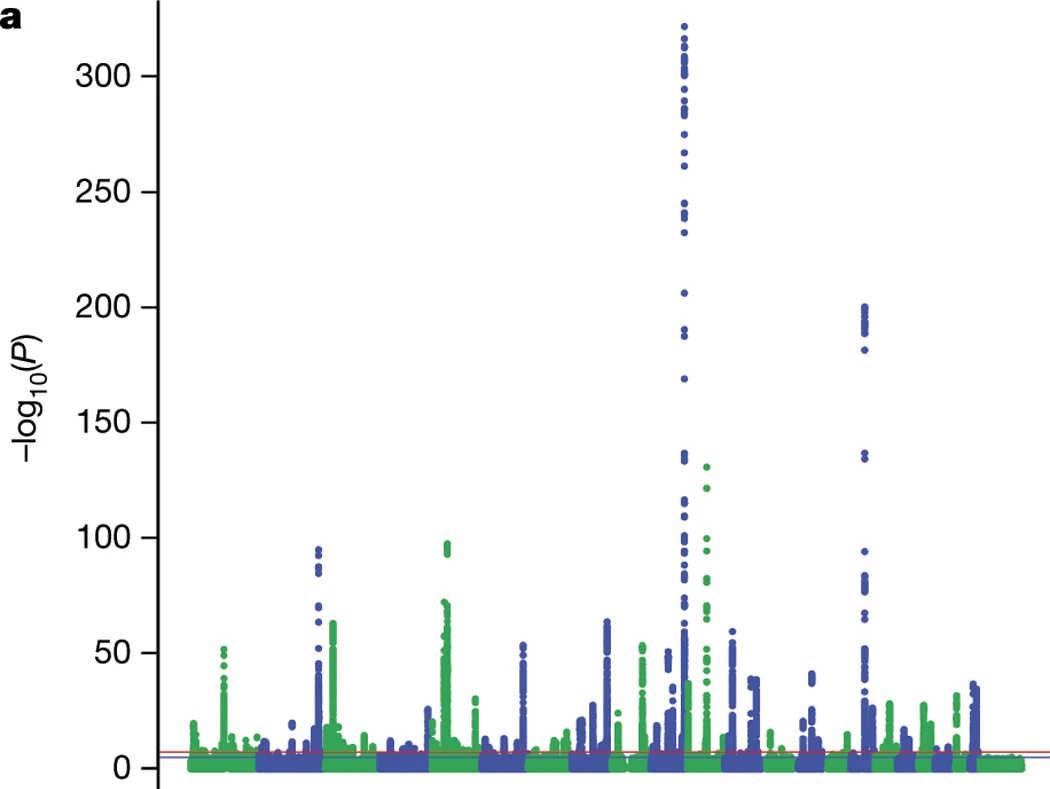
\includegraphics[width=0.5\textwidth]{\presentationgoldparispath/41586_2017_Article_BFnature24284_Fig1_HTML.jpg}
            \end{center}
            \caption{Genetic variant associations with breast cancer risk (DOI:10.1038/nature24284).}
        \end{figure}

    \end{frame}

%%%%%%%%%%%%%%%%%%%%%%%%%%%%%%%%%%%%%%%%%%%%%%%%%%%%%%%%%%%%%%%%%%%%%%%%%%%%%%%%
    \begin{frame}
        \frametitle{Effect of genetic variants on gene expression: eQTLs}

        \begin{itemize}
            \item Quantitative trait loci (QTL) variants associated with changes of quantitative phenotypes
            \item Expression (eQTL) are variants associated with changes of gene expression in a given tissue
            \item eQTLs provide a putative molecular mechanism of a variant
        \end{itemize}

        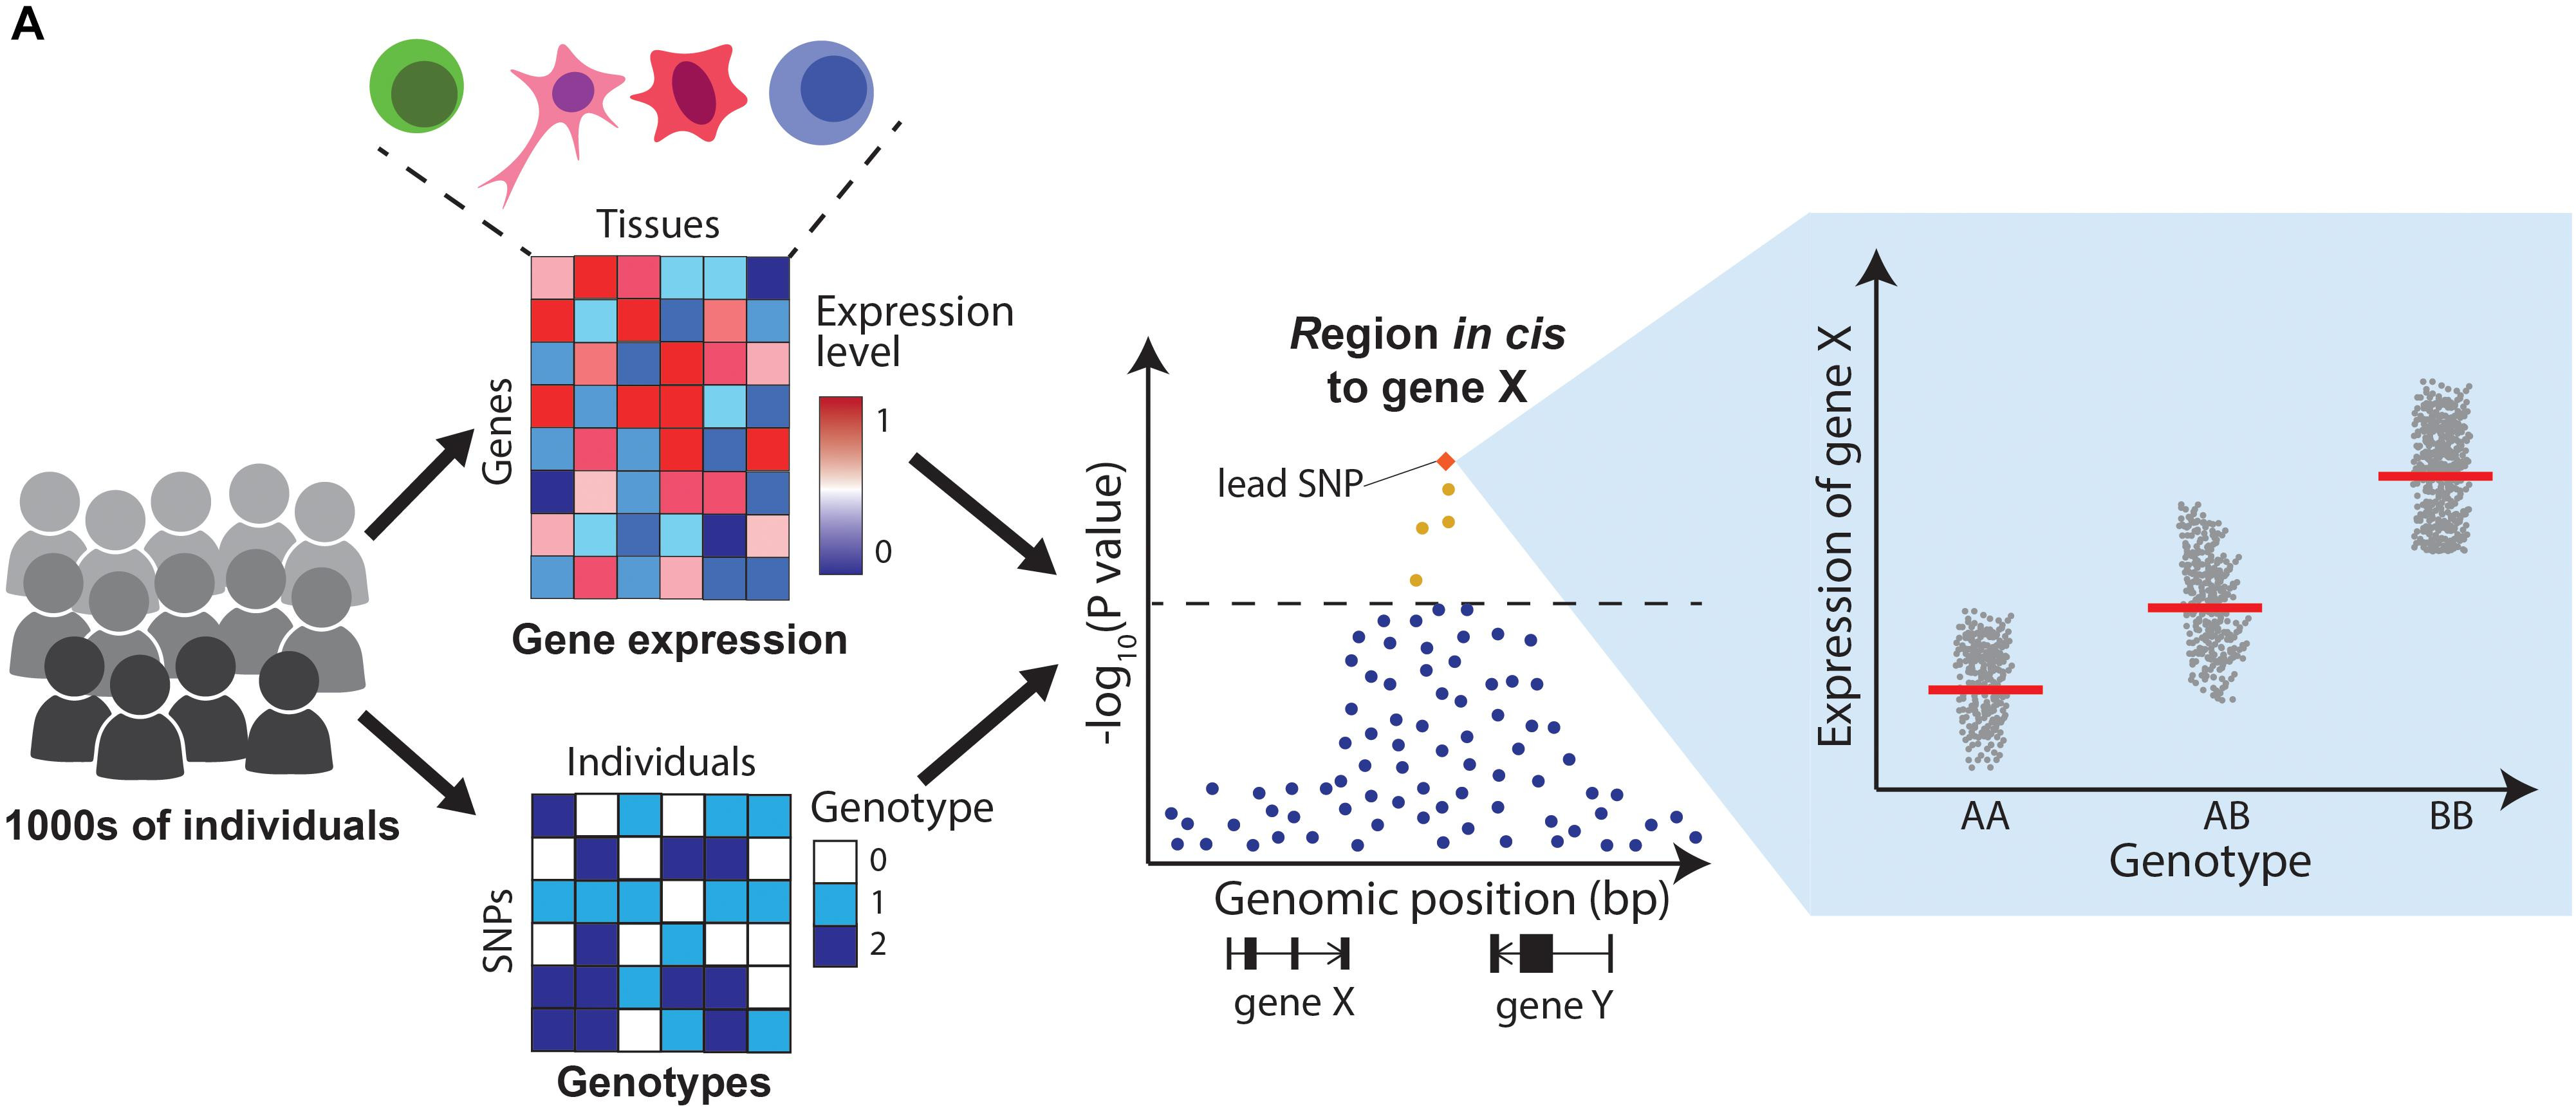
\includegraphics[width=0.7\textwidth]{\presentationgoldparispath/doi_10.3389_fgene.2020.00424_fig4a.jpg}

        \let\thefootnote\relax\footnotetext{Cano-Gamez et al. 2020. doi:10.3389/fgene.2020.00424}
    \end{frame}

%%%%%%%%%%%%%%%%%%%%%%%%%%%%%%%%%%%%%%%%%%%%%%%%%%%%%%%%%%%%%%%%%%%%%%%%%%%%%%%%
    \begin{frame}
        \frametitle{Annotation of eQTLs traits using colocalization analysis}

        \begin{center}
            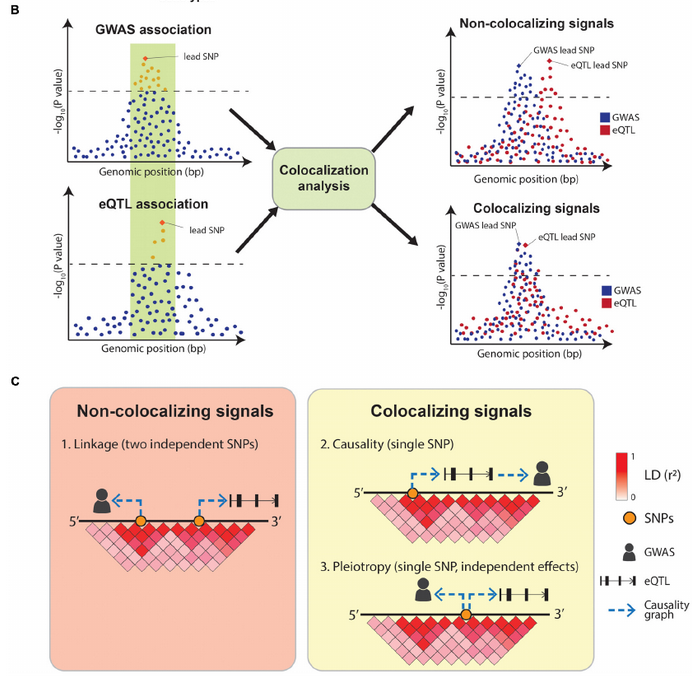
\includegraphics[width=0.6\textwidth]{\presentationgoldparispath/doi_10.3389_fgene.2020.00424_fig4bc.png}
        \end{center}

        \let\thefootnote\relax\footnotetext{Cano-Gamez et al. 2020. doi:10.3389/fgene.2020.00424}
    \end{frame}

%%%%%%%%%%%%%%%%%%%%%%%%%%%%%%%%%%%%%%%%%%%%%%%%%%%%%%%%%%%%%%%%%%%%%%%%%%%%%%%%
    \begin{frame}
        \frametitle{Pleiotropic genetic variants}

        \begin{itemize}
            \item Large datasets of associations have shown that many genetic variants change simultaneously susceptibility to many diseases, for instance:
        \end{itemize}

        % full size table is table
        \begin{table}[!tbp]
            \centering
            \scriptsize

            \csvreader[separator=tab,
            tabular=crcp{0.4\textwidth},
            late after last line=\\\hline,
            head,
            table head=\\\hline \bfseries Chrom. & \bfseries Pos (hg38) & \bfseries Gene marker& \bfseries Trait categories\\\hline,
            ]{\mspath/cmpt_count_per_rsid.py/count_per_rsid_gwas_ms.tsv}{}% use head of csv as column names
                {\csvcoli\ & \csvcolii\ & \csvcolv\ & \csvcolvi}% specify your coloumns here
            \vspace{15pt}\label{tab:pleitropic_variants}
        \end{table}

    \end{frame}

%%%%%%%%%%%%%%%%%%%%%%%%%%%%%%%%%%%%%%%%%%%%%%%%%%%%%%%%%%%%%%%%%%%%%%%%%%%%%%%%
    \begin{frame}
        \frametitle{Summary of previous and my work here}

        \begin{center}
            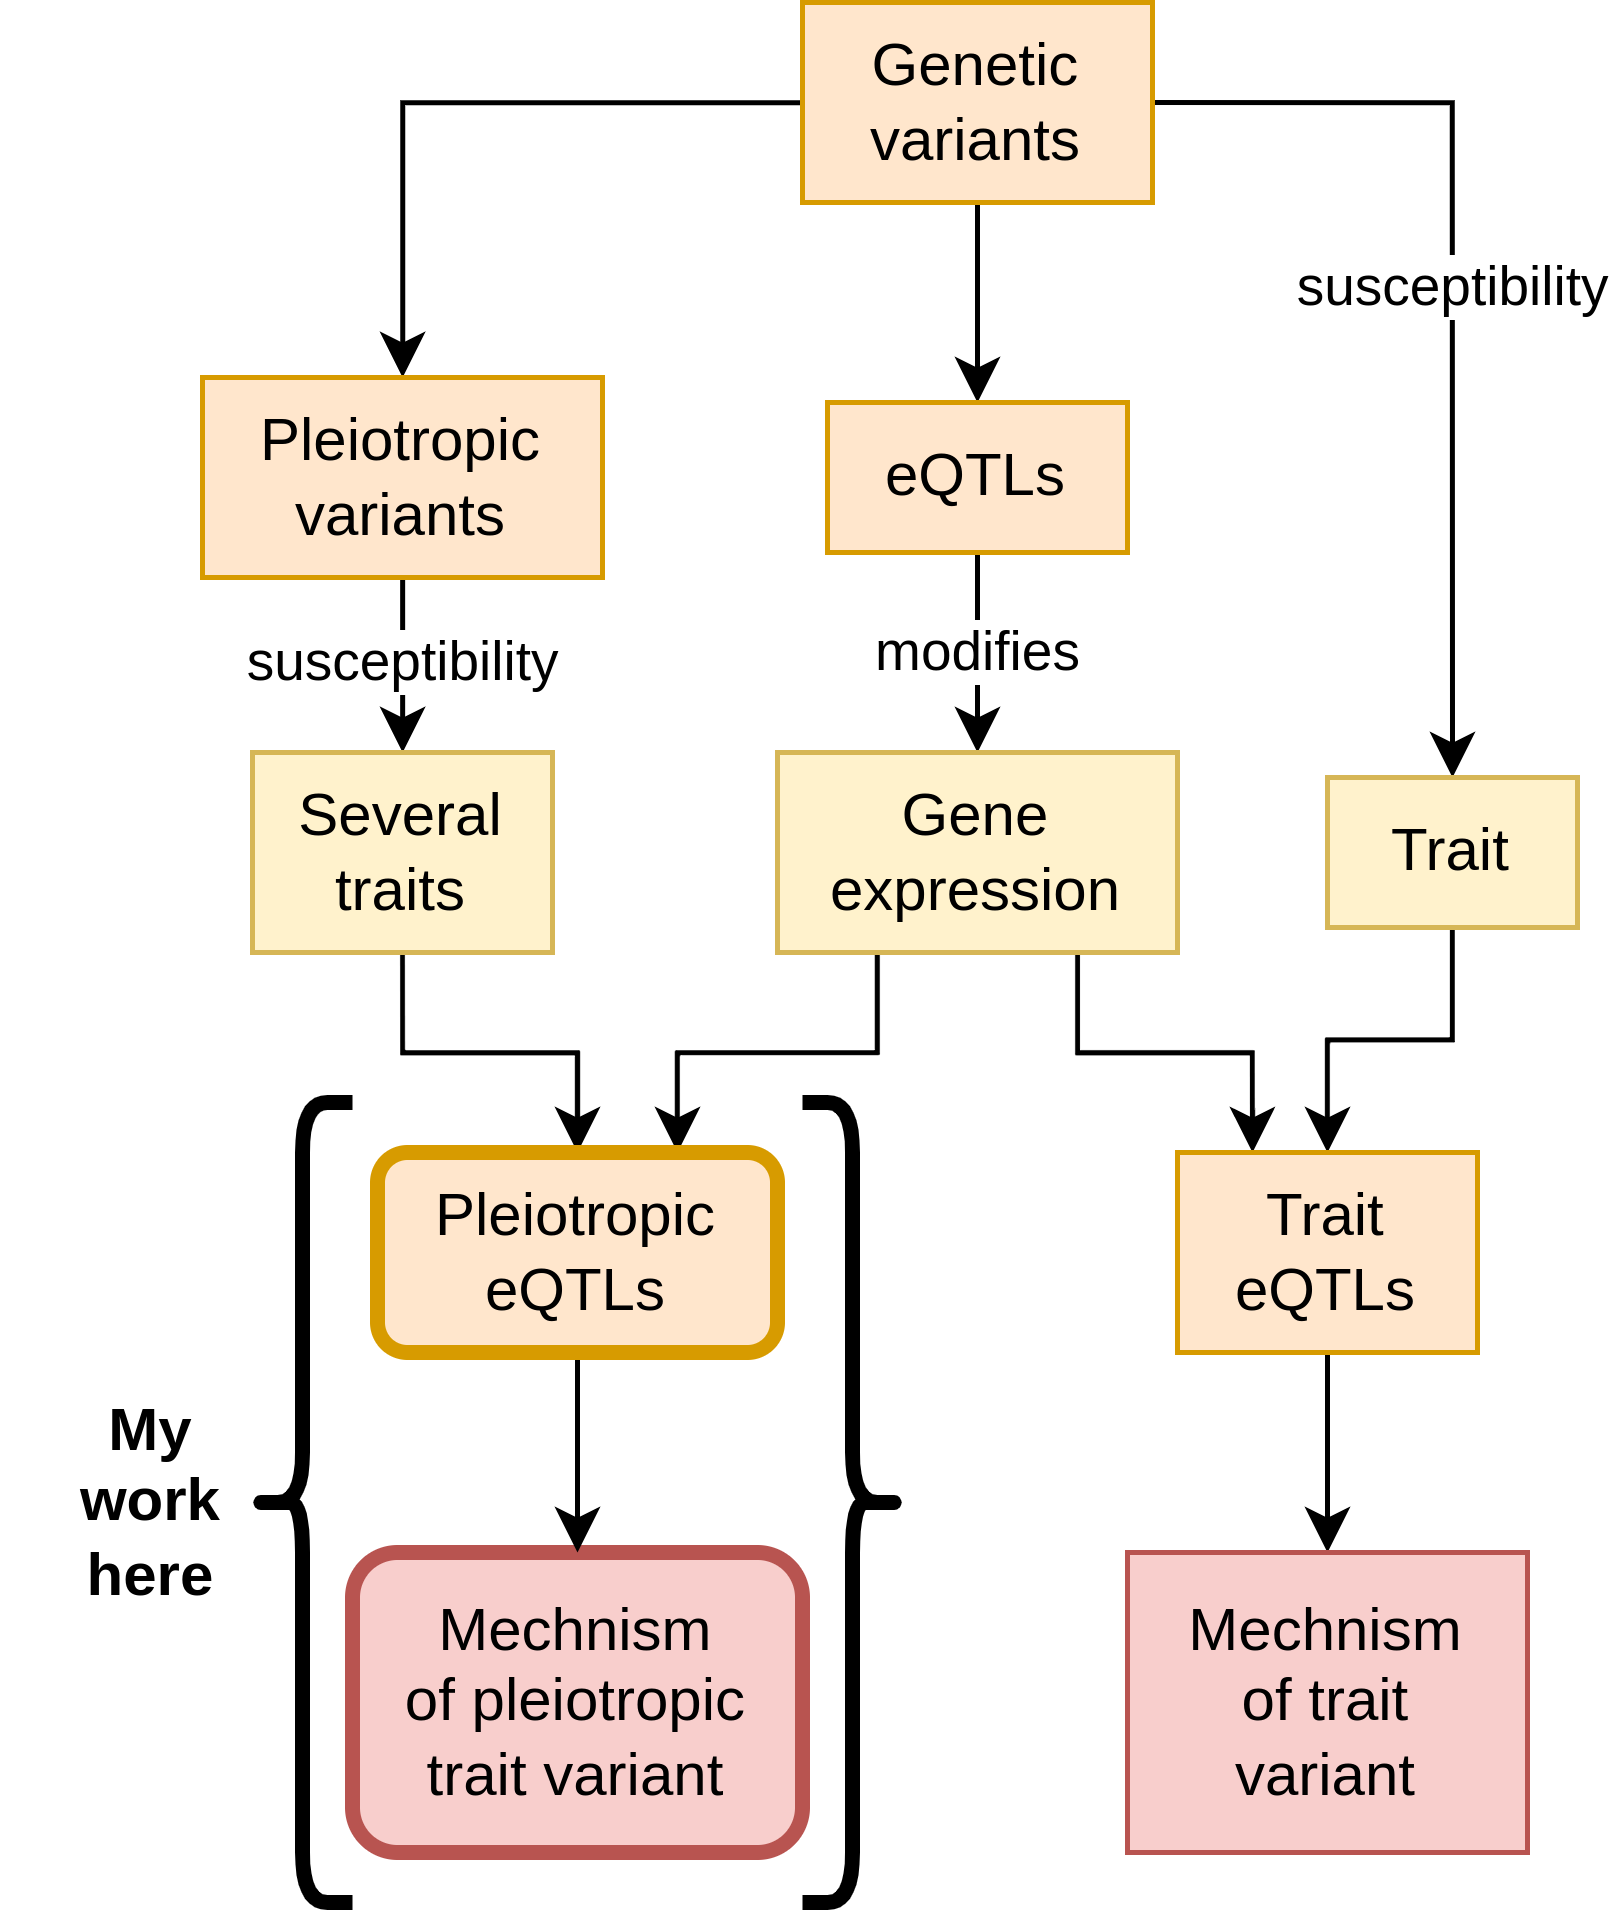
\includegraphics[width=0.6\textwidth]{fig/graphical_intro_approach.drawio.png}
        \end{center}

    \end{frame}

%%%%%%%%%%%%%%%%%%%%%%%%%%%%%%%%%%%%%%%%%%%%%%%%%%%%%%%%%%%%%%%%%%%%%%%%%%%%%%%%
    \begin{frame}
        \frametitle{Strategy}

        \begin{enumerate}
            \item Compute colocalization of eQTLs and GWAS variants
            \item Split eQTLs by the number of associated disease categories
            \item Compare molecular properties of pleiotropic eQTLs
        \end{enumerate}

    \end{frame}


    \section{Results} %%%%%%%%%%%%%%%%%%%%%%%%%%%%%%%%%%%%%%%%%%%%%%%%%%%%%%%%%%%%%%

%%%%%%%%%%%%%%%%%%%%%%%%%%%%%%%%%%%%%%%%%%%%%%%%%%%%%%%%%%%%%%%%%%%%%%%%%%%%%%%%
    \begin{frame}
        \frametitle{Most pleiotroic eQTLs}

        \begin{itemize}
            \item Example pleiotropic eQTLs in different cytobands
            \item The representative gene is the eQTL gene with the highest PubMed publication count
        \end{itemize}

% full size table is table
        \begin{table}[!tbp]
            \centering
            \scriptsize

            \csvreader[separator=tab,
            tabular=crcp{0.4\textwidth},
            late after last line=\\\hline,
            head,
            table head=\\\hline \bfseries Chrom. & \bfseries Pos (hg38) & \bfseries Gene marker& \bfseries Trait categories\\\hline,
            ]{\mspath/cmpt_count_per_rsid.py/count_per_rsid_gwas_ms.tsv}{}% use head of csv as column names
                {\csvcoli\ & \csvcolii\ & \csvcolv\ & \csvcolvi}% specify your coloumns here
            \vspace{15pt}\label{tab:pleitropic_variants}
        \end{table}

    \end{frame}

%%%%%%%%%%%%%%%%%%%%%%%%%%%%%%%%%%%%%%%%%%%%%%%%%%%%%%%%%%%%%%%%%%%%%%%%%%%%%%%%
    \begin{frame}
        \frametitle{Is the effect size of pleiotropic eQTLs different?}

        \begin{figure}[!ht]

            \begin{subfigure}[]{.49\textwidth}
                \textbf{a}
                \\
                \includegraphics[width=\textwidth]{\mspath/pltbar_x_per_gwas_cat_y_beta_neglog10pval.py/eqtl_beta.png}
            \end{subfigure}
            %
            \begin{subfigure}[]{.49\textwidth}
                \textbf{b}
                \\
                \includegraphics[width=\textwidth]{\mspath/pltbar_x_per_gwas_cat_y_beta_neglog10pval.py/gwas_beta.png}
            \end{subfigure}

        \end{figure}
        %
        \vfill
        Yes, pleiotropic eQTLs have a lower effect on gene expression and traits

    \end{frame}

%%%%%%%%%%%%%%%%%%%%%%%%%%%%%%%%%%%%%%%%%%%%%%%%%%%%%%%%%%%%%%%%%%%%%%%%%%%%%%%%
    \begin{frame}
        \frametitle{Are pleiotropic eQTLs closer to genes?}

        \begin{center}
            \includegraphics[width=0.5\textwidth]{\mspath/plt_x_per_variant_y_egene_distance.py/violin.png}
        \end{center}
        \vfill
        Yes, distance to genes decreases with the pleiotropy

    \end{frame}

%%%%%%%%%%%%%%%%%%%%%%%%%%%%%%%%%%%%%%%%%%%%%%%%%%%%%%%%%%%%%%%%%%%%%%%%%%%%%%%%
    \begin{frame}
        \frametitle{Are pleiotropic eQTLs associated to more genes?}

        \begin{center}
            \includegraphics[width=0.5\textwidth]{\mspath/pltbar_x_per_variant_etissue_y_egene.py/plt.png}
        \end{center}
        \vfill
        Yes, number of target gene increaseas with the pleiotropy

    \end{frame}

%%%%%%%%%%%%%%%%%%%%%%%%%%%%%%%%%%%%%%%%%%%%%%%%%%%%%%%%%%%%%%%%%%%%%%%%%%%%%%%%
    \begin{frame}
        \frametitle{A web portal to access the eQTL/trait annotations}

        \url{https://gwas2eqtl.tagc.univ-amu.fr/gwas2eqtl}

        \begin{center}
            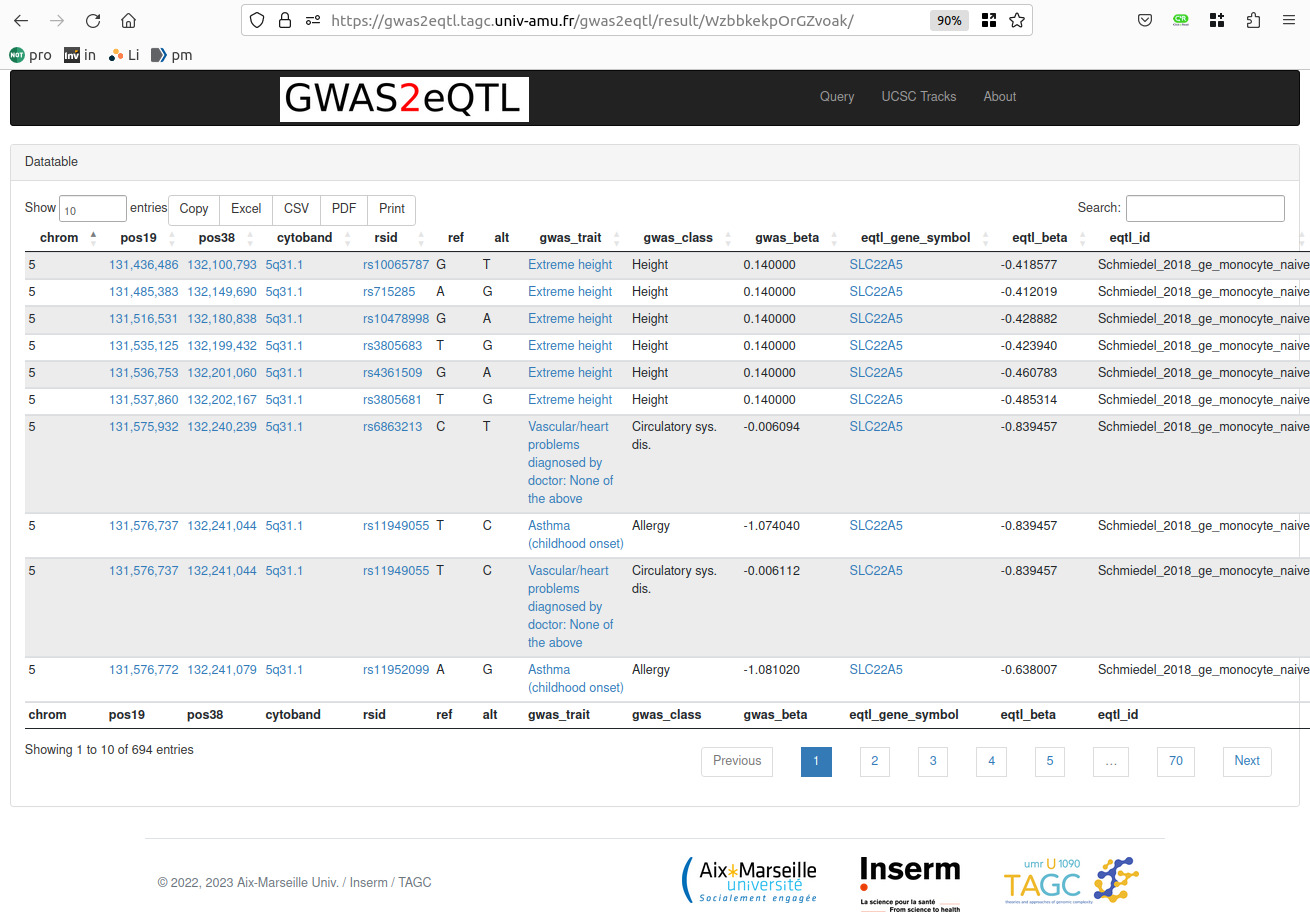
\includegraphics[width=0.9\textwidth]{fig/gwas2eqtl.png}
        \end{center}

    \end{frame}

%%%%%%%%%%%%%%%%%%%%%%%%%%%%%%%%%%%%%%%%%%%%%%%%%%%%%%%%%%%%%%%%%%%%%%%%%%%%%%%%
    \begin{frame}
        \frametitle{Summary of my work}

        \begin{center}
            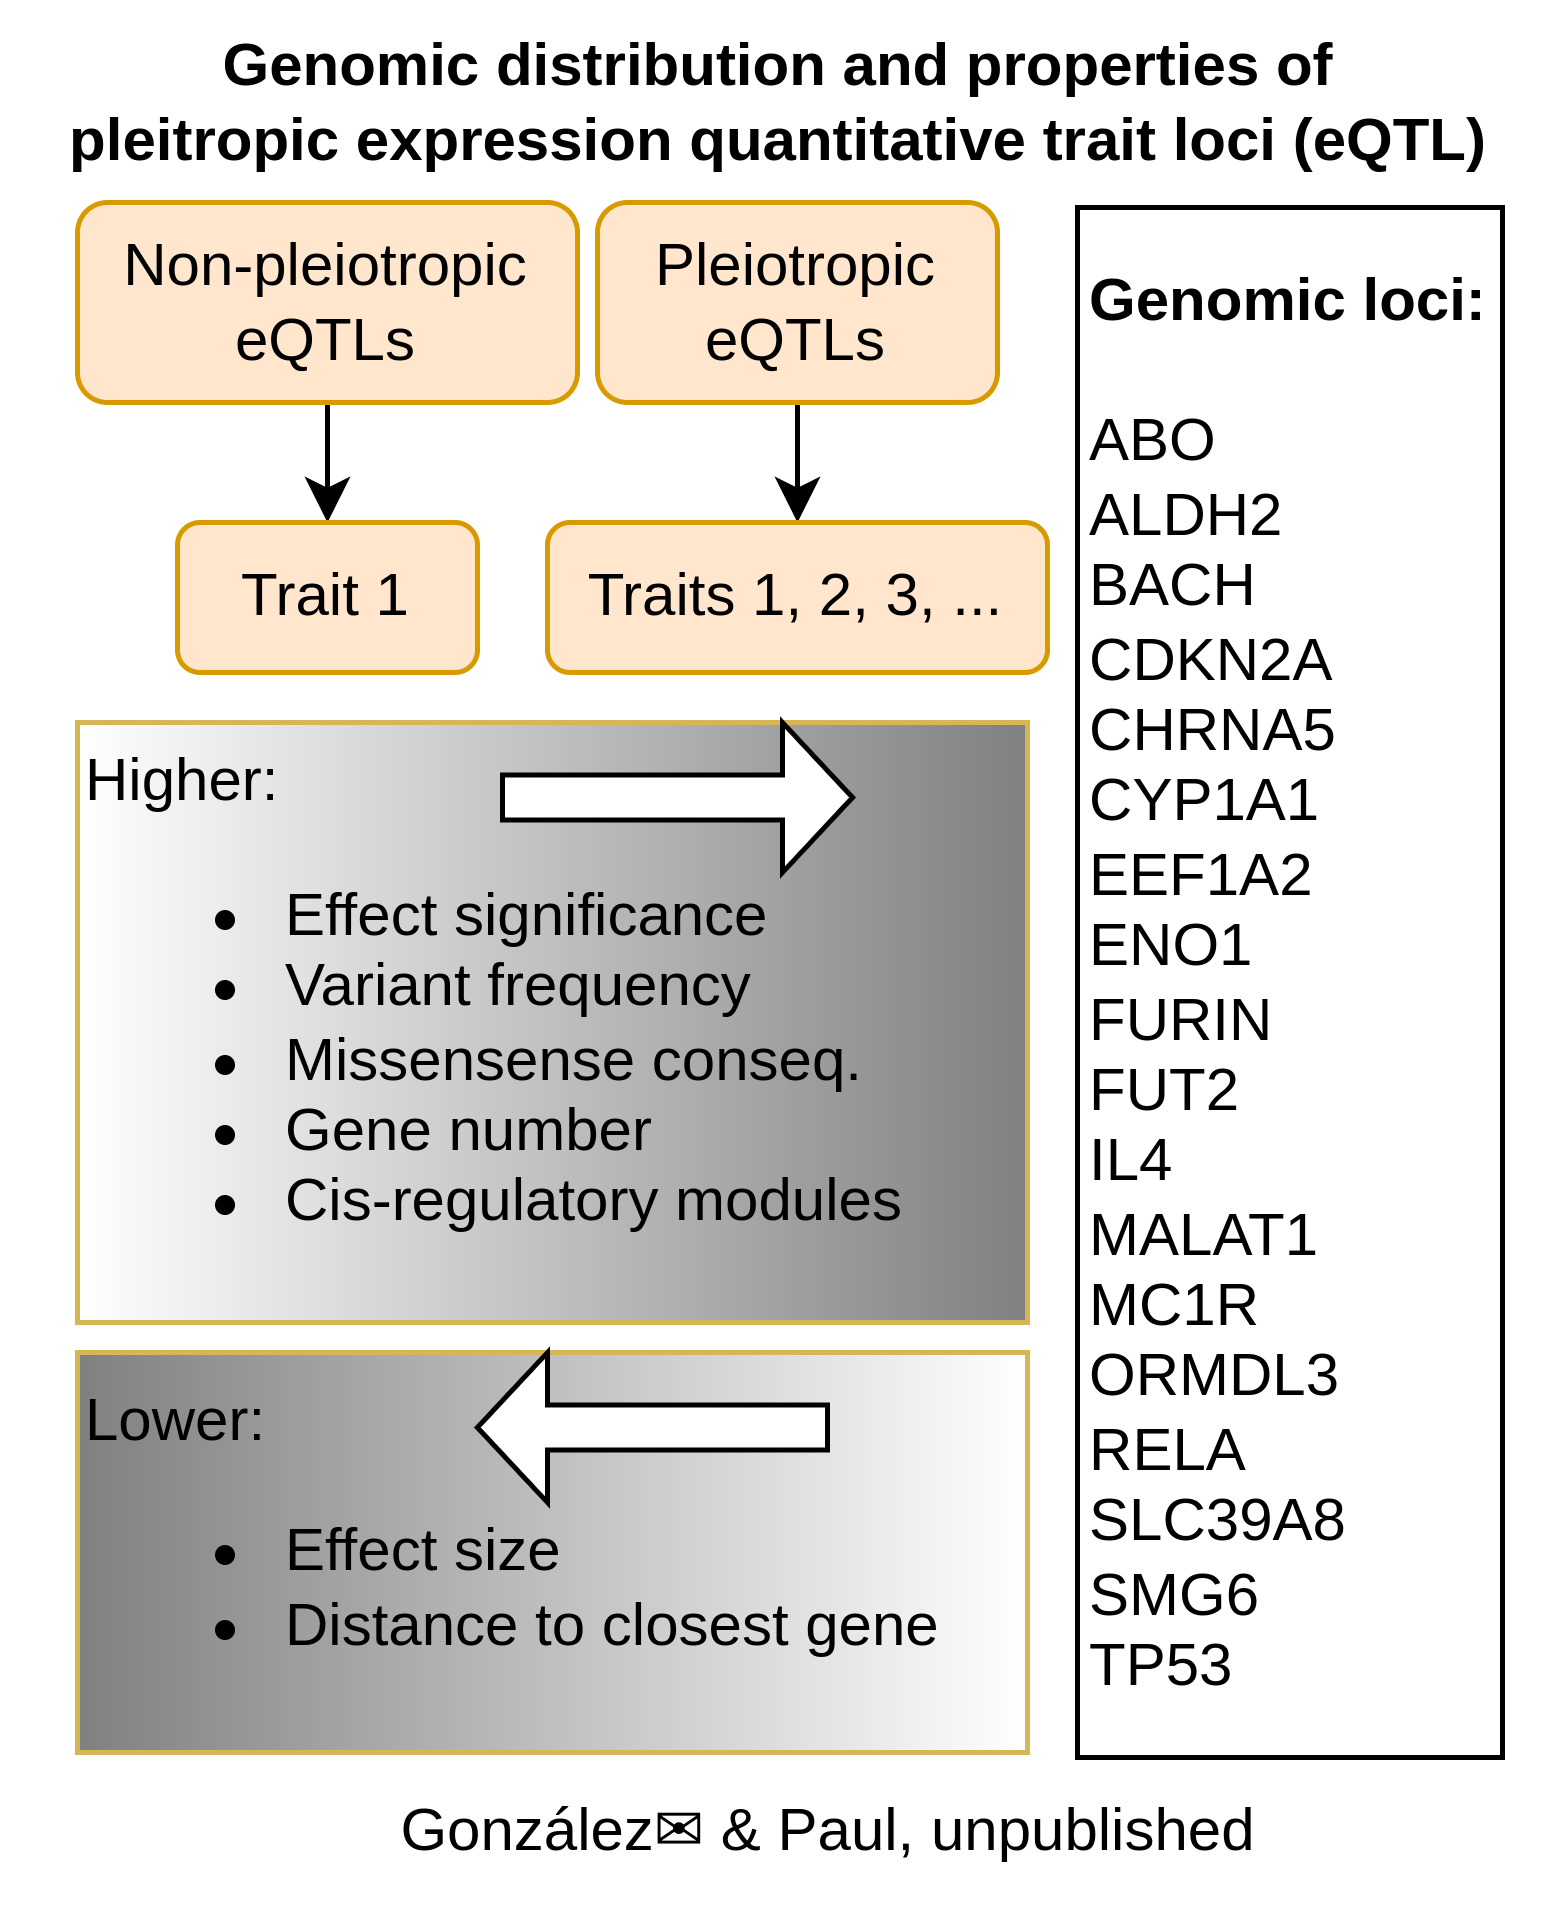
\includegraphics[width=0.5\textwidth]{fig/graphical_abstract.drawio.png}
        \end{center}

    \end{frame}

%%%%%%%%%%%%%%%%%%%%%%%%%%%%%%%%%%%%%%%%%%%%%%%%%%%%%%%%%%%%%%%%%%%%%%%%%%%%%%%%
    \begin{frame}
        \frametitle{Acknowledgements}

        \begin{itemize}
            \item P Paul
            \item L Lecerf (M1), P Rihet, M Michel, S Marquet, S Spicuglia
        \end{itemize}
%
        \vfill
%
        Funding
%
        \begin{itemize}
            \item Institut Cancer et Immunologie - Aix-Marseille Univ.
            \item Agence nationale de la recherche (ANR)
            \item Centre de Calcul Intensif d'Aix-Marseille
        \end{itemize}

    \end{frame}

\end{document}
